\documentclass[a4paper,11pt]{report}
\usepackage[utf8]{inputenc}
\usepackage[T1]{fontenc}
\usepackage{lmodern}
\usepackage[ngerman]{babel}
\usepackage[margin=20mm, left=20mm, right=10mm, headheight=15pt, includeheadfoot]{geometry}
\usepackage{fancyhdr}
\usepackage{opensans}
\usepackage{titlesec}
\usepackage{tocloft}
\usepackage{titling}
\usepackage{hyperref}
\usepackage{graphicx}
\usepackage{enumerate}
\usepackage{float}
\usepackage{caption}
\usepackage{listings}
\usepackage{minted}
\usepackage{subcaption}
\usepackage{enumitem}
\usemintedstyle{vs}

% Author and subject
\author{Felix Hillebrand}
\newcommand{\subject}{SSD4UE}

\graphicspath{ {./images/} }

% Set default font to OpenSans
\renewcommand*\familydefault{\sfdefault}

% Page style for cover page
\fancypagestyle{cover}{
    \fancyhf{}
    \renewcommand{\headrulewidth}{0pt}
    \renewcommand{\footrulewidth}{0pt}
}

% Page style for main content
\fancypagestyle{main}{
    \fancyhf{}
    \fancyhead[L]{\theauthor}
    \fancyhead[R]{\subject}
    \fancyfoot[C]{\thepage}
    \renewcommand{\headrulewidth}{0.4pt}
    \renewcommand{\footrulewidth}{0pt}
}

\titleformat{\chapter}[block]
  {\normalfont\Large\bfseries} % change \Large to \large or any other size that fits
  {\thechapter}
  {1em}
  {}

  \titlespacing*{\chapter}{0pt}{*4}{*2.5}

% Cover page
\newcommand{\coverpage}{
    \thispagestyle{cover}
    \begin{center}
        % {
\includegraphics[height=3cm]{fh-logo.png}}\\[1cm]
        {\LARGE \thetitle}\\[0.5cm]
        {\large \theauthor}\\
        \href{mailto:97hilfel@gmail.com}{97hilfel@gmail.com}\\
    \end{center}
    \tableofcontents
    \clearpage
}

\newcommand{\screenshot}[1]{
    \begin{figure}[H]
        \centering
        \includegraphics[scale=0.375]{#1}
    \end{figure}
}

% Main document
\begin{document}

% Color definitions
\definecolor{LightGray}{gray}{0.9}
\definecolor{DarkGray}{gray}{0.3}

\title{Subject~-~Exercise}
\coverpage

\pagenumbering{roman}
\clearpage
\pagenumbering{arabic}
\pagestyle{main}

\chapter{Python}
    \begin{description}
        \item[Aufgabe:] Vervollständigen Sie folgende Python Funktionen (g ist ein networkx Graph) \hfill
        \item[Lösung:] \hfill \newline % Use hfill to move the figure to the next line
            \begin{minted}[
                frame=lines,
                framesep=2mm,
                baselinestretch=1.2,
                bgcolor=LightGray,
                linenos,
                breaklines
                ]{python}
#prints all nodes in g in alphabetical order 
def print_all_nodes(g):
    for node in sorted(g.nodes()):
        print(node)

#adds the nodes start, start+1, start+2,....start+count-1 to the grapgh g 
def add_nodes_(g, start, count):
    g.add_nodes_from([i for i in range(start, start + count)])

#adds the nodes start, start+1, start+2,....start+count-1 to the graph 
#as well as every possible edge between the new nodes 
def add_nodes_connected(g, start, count):
    new_nodes = list(range(start, start + count))
    for i in range(len(new_nodes)):
        for j in range(i + 1, len(new_nodes)):
            g.add_edge(new_nodes[i], new_nodes[j])
            \end{minted}

        \item[Tests:] \hfil \newline
        \begin{minted}[
            frame=lines,
            framesep=2mm,
            baselinestretch=1.2,
            bgcolor=LightGray,
            linenos,
            breaklines
        ]{python}
g = nx.Graph()
add_nodes_(g, 0, 5)
print_all_nodes(g)

# Plot graph for better visualization
nx.draw(g, with_labels=True)
plt.show()
        \end{minted}
        Output: 
        \begin{minted}[
            frame=lines,
            framesep=2mm,
            baselinestretch=1.2,
            bgcolor=LightGray,
            linenos,
            breaklines
        ]{text}
0
1
2
3
4
        \end{minted}

        \screenshot{notebook/assets/aufgabe_01_nodes.png}

        \begin{minted}[
            frame=lines,
            framesep=2mm,
            baselinestretch=1.2,
            bgcolor=LightGray,
            linenos,
            breaklines
        ]{python}
g = nx.Graph()
add_nodes_connected(g, 0, 5)
print_all_nodes(g)

# Plot graph for better visualization
nx.draw(g, with_labels=True)
plt.show()
        \end{minted}
        Output: 
        \begin{minted}[
            frame=lines,
            framesep=2mm,
            baselinestretch=1.2,
            bgcolor=LightGray,
            linenos,
            breaklines
        ]{text}
0
1
2
3
4
        \end{minted}
        \screenshot{notebook/assets/aufgabe_01_connected.png}
    \end{description}
\newpage

\chapter{Darstellung}
\begin{description}
    \item[Aufgabe:] Zeichnen Sie den folgenden Graphen \newline
        \begin{math}
            G = (V, E), V = \{a, b, c, d, e\}, E = \{\{a, b\}, \{a, d\}, \{c, e\}, \{b, c\}, \{e, d\}\}
        \end{math}
    \item[Lösung:] \hfill \newline % Use hfill to move the figure to the next line
        \begin{minted}[
            frame=lines,
            framesep=2mm,
            baselinestretch=1.2,
            bgcolor=LightGray,
            linenos,
            breaklines
            ]{python}
# Step 1: Create a graph
g = nx.Graph()
g.add_edges_from([('a', 'b'), ('a', 'd'), ('c', 'e'), ('b', 'c'), ('e', 'd')])

# Step 2: Convert to AGraph (Graphviz graph)
a = to_agraph(g)

# Step 3: Draw using AGraph
a.draw("assets/aufgabe_02_graph.png", format="png", prog="dot")

# Step 4: Display the result
display(Image(filename="assets/aufgabe_02_graph.png"))
        \end{minted}
        \screenshot{notebook/assets/aufgabe_02_graph.png}
\end{description}
\newpage

\chapter{Wanderungen, Wege, Pfade}
Gegeben Sei nachfolgende Darstelling eines Graphen mit 8 Knoten

\begin{enumerate}
    \item Geben Sie alle möglichen \textit{Wege} von 1 nach 8 an.
    \item Sind die nachfolgenden Kantenfolgen $W_1$ bis $W_6$ Wanderungen, Wege oder Pfade?
\end{enumerate}

\begin{enumerate}
    % First main item
    \item \label{item:backrefA} \hfill % Use hfill to move the figure to the next line
    \begin{description}
        \item[Aufgabe:] 
         \hfill
        \item[Lösung:] \hfill \newline % Use hfill to move the figure to the next line
            Solution
    \end{description}
\end{enumerate}
\newpage


\chapter{Teilgraph}

Gegeben sei der Graph aus Punkt 2. bestemmen Sie jeweils ob die Graphen $H_1$ bis $H_4$ Teilgraphen sind.
\begin{itemize}
    \item $G = (\{a, b, c, d, e\}, \{\{a, b\}, \{a, d\}, \{c, e\}, \{b, c\}, \{e, d\}\})$
    \begin{figure}[htbp]
        \centering
        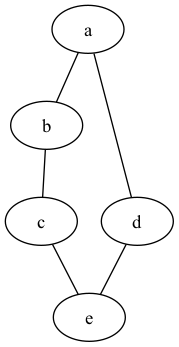
\includegraphics[width=3cm]{notebook/assets/aufgabe_02_graph.png}
        \caption{Graph $G$}
        \label{fig:graph_h_1}
    \end{figure}
    \item $H_1 = (\{ a, b, d\}, \{ \{a, b\}, \{a, d\}\})$ 
    \begin{figure}[htbp]
        \centering
        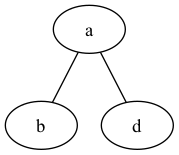
\includegraphics[width=3cm]{notebook/assets/aufgabe_04_h1.png}
        \caption{Graph $H_1$}
        \label{fig:graph_h_1}
    \end{figure}
    \item $H_2 = (\{ a, b, c, d, e\}, \{ \{a, b\}, \{a, d\}, \{b, c\}, \{d, e\}\})$
    \begin{figure}[htbp]
        \centering
        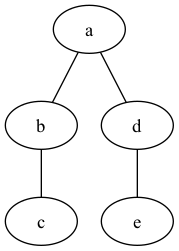
\includegraphics[width=3cm]{notebook/assets/aufgabe_04_h2.png}
        \caption{Graph $H_2$}
        \label{fig:graph_h_2}
    \end{figure}
    \item $H_3 = (\{ a, b, f\}, \{ \{a, b\}\})$
    \begin{figure}[htbp]
        \centering
        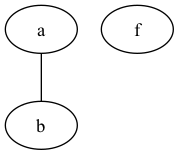
\includegraphics[width=3cm]{notebook/assets/aufgabe_04_h3.png}
        \caption{Graph $H_3$}
        \label{fig:graph_h_3}
    \end{figure}
    \item $H_3 = (\{ d, e\},\emptyset)$
    \begin{figure}[htbp]
        \centering
        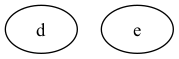
\includegraphics[width=3cm]{notebook/assets/aufgabe_04_h4.png}
        \caption{Graph $H_4$}
        \label{fig:graph_h_4}
    \end{figure}
\end{itemize}

\begin{figure}
    \centering
    \begin{minted}[
        frame=lines,
        framesep=2mm,
        baselinestretch=1.2,
        bgcolor=LightGray,
        linenos,
        breaklines
        ]{python}
def is_subgraph(small, big):
"""Check if small is a subgraph of big in the mathematical sense."""
# Check if all nodes of small are in big
if not set(small.nodes()).issubset(set(big.nodes())):
    return False
# Check if all edges of small are in big
if not set(small.edges()).issubset(set(big.edges())):
    return False
return True

# graph definition obmitted for brevity

graphs = [h1, h2, h3, h4]
titles = ["h1", "h2", "h3", "h4"]

# render graphs
for idx, (graph, title) in enumerate(zip(graphs, titles), 1):
    a = to_agraph(graph)
    filename = f"assets/{prefix}_h{idx}.png"
    # Draw using AGraph
    a.draw(filename, format="png", prog="dot")
    # Display the result
    display(Image(filename=filename))

for i in range(len(graphs)):
    if is_subgraph(graphs[j], G):
        print(f"{titles[i]} is a subgraph of G")
    \end{minted}
    \caption{Python Code für Grafiken und check}
    \label{fig:is_subgraph}
\end{figure}

\begin{figure}
    \centering
    \begin{minted}[
        frame=lines,
        framesep=2mm,
        baselinestretch=1.2,
        bgcolor=LightGray,
        linenos,
        breaklines
        ]{text}
h1 is a subgraph of G
h2 is a subgraph of G
h3 is a subgraph of G
h4 is a subgraph of G
    \end{minted}
    \caption{Python Code Ausgabe}
    \label{fig:is_subgraph_output}
\end{figure}

\newpage

\chapter{Visualisierung}

Stellen Sie das folgende Programm als Kontrollflussgraph dar. 

\begin{minted}[
    frame=lines,
    framesep=2mm,
    baselinestretch=1.2,
    bgcolor=LightGray,
    linenos,
    breaklines
    ]{java}
while (a < b) {
    if (a % c == 0) break;
    a++;
}
\end{minted}

\begin{figure}[htbp]
    \centering
    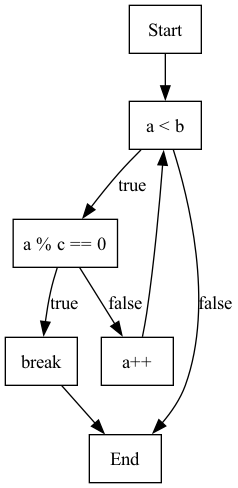
\includegraphics[width=3cm]{notebook/assets/aufgabe_05_graph.png}
    \caption{Control flow path}
    \label{fig:program_graph}
\end{figure}


\newpage

\chapter{Zustandsgraphen}



\newpage

\chapter{Eulerkreis}

Implementieren Sie den Fleury Algorithmus aus dem Skriptum und finden Sie einen Eulerkreis in folgendem Graph:
\begin{figure}[htbp]
    \centering
    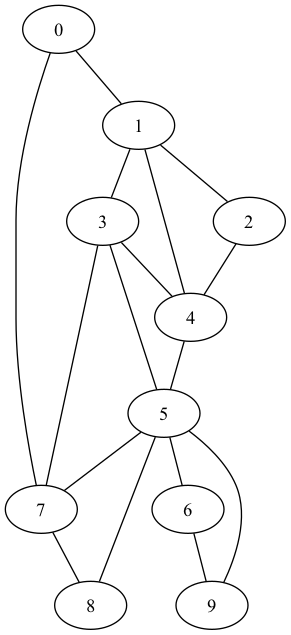
\includegraphics[width=3cm]{notebook/assets/aufgabe_07_graph.png}
    \caption{Graph}
    \label{fig:eulerkreis_graph}
\end{figure}

Als Output gib die Zustände der Variablen $v$, $F$, $e$ und $k$ vor jeder Iteration der Schleife an.

\begin{minted}[
    frame=lines,
    framesep=2mm,
    baselinestretch=1.2,
    bgcolor=LightGray,
    linenos,
    breaklines
    ]{text}
idx 0 - v 3 - F [(0, 1), (0, 7), (1, 2), (1, 3), (1, 4), (2, 4), (3, 4), (3, 7), (3, 5), (4, 5), (5, 7), (5, 8), (5, 6), (5, 9), (6, 9), (7, 8)] - e (3, 7) - K [3]
idx 1 - v 7 - F [(0, 1), (0, 7), (1, 2), (1, 3), (1, 4), (2, 4), (3, 4), (3, 5), (4, 5), (5, 7), (5, 8), (5, 6), (5, 9), (6, 9), (7, 8)] - e (7, 0) - K [3, 7]
idx 2 - v 0 - F [(0, 1), (1, 2), (1, 3), (1, 4), (2, 4), (3, 4), (3, 5), (4, 5), (5, 7), (5, 8), (5, 6), (5, 9), (6, 9), (7, 8)] - e (0, 1) - K [3, 7, 0]
idx 3 - v 1 - F [(1, 2), (1, 3), (1, 4), (2, 4), (3, 4), (3, 5), (4, 5), (5, 7), (5, 8), (5, 6), (5, 9), (6, 9), (7, 8)] - e (1, 2) - K [3, 7, 0, 1]
idx 4 - v 2 - F [(1, 3), (1, 4), (2, 4), (3, 4), (3, 5), (4, 5), (5, 7), (5, 8), (5, 6), (5, 9), (6, 9), (7, 8)] - e (2, 4) - K [3, 7, 0, 1, 2]
idx 5 - v 4 - F [(1, 3), (1, 4), (3, 4), (3, 5), (4, 5), (5, 7), (5, 8), (5, 6), (5, 9), (6, 9), (7, 8)] - e (4, 1) - K [3, 7, 0, 1, 2, 4]
idx 6 - v 1 - F [(1, 3), (3, 4), (3, 5), (4, 5), (5, 7), (5, 8), (5, 6), (5, 9), (6, 9), (7, 8)] - e (1, 3) - K [3, 7, 0, 1, 2, 4, 1]
idx 7 - v 3 - F [(3, 4), (3, 5), (4, 5), (5, 7), (5, 8), (5, 6), (5, 9), (6, 9), (7, 8)] - e (3, 4) - K [3, 7, 0, 1, 2, 4, 1, 3]
idx 8 - v 4 - F [(3, 5), (4, 5), (5, 7), (5, 8), (5, 6), (5, 9), (6, 9), (7, 8)] - e (4, 5) - K [3, 7, 0, 1, 2, 4, 1, 3, 4]
idx 9 - v 5 - F [(3, 5), (5, 7), (5, 8), (5, 6), (5, 9), (6, 9), (7, 8)] - e (5, 3) - K [3, 7, 0, 1, 2, 4, 1, 3, 4, 5]    
\end{minted}
\begin{figure}[htbp]
    \centering
    \begin{subfigure}[b]{0.3\textwidth}
        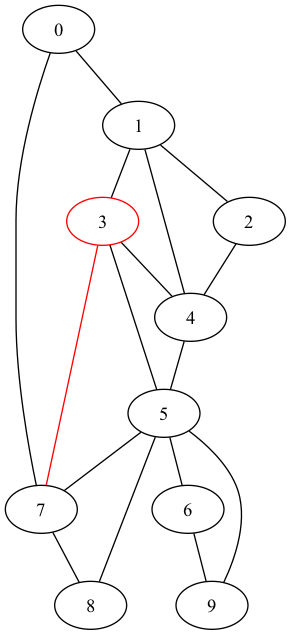
\includegraphics[height=0.29\textheight]{notebook/assets/aufgabe_07_fleury_step_0.png}
        \caption{Step 1}
        \label{fig:fleury_step_1}
    \end{subfigure}
    \hfill
    \begin{subfigure}[b]{0.3\textwidth}
        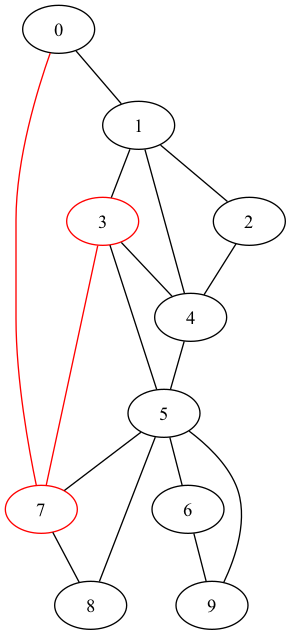
\includegraphics[height=0.29\textheight]{notebook/assets/aufgabe_07_fleury_step_1.png}
        \caption{Step 2}
        \label{fig:fleury_step_2}
    \end{subfigure}
    \hfill
    \begin{subfigure}[b]{0.3\textwidth}
        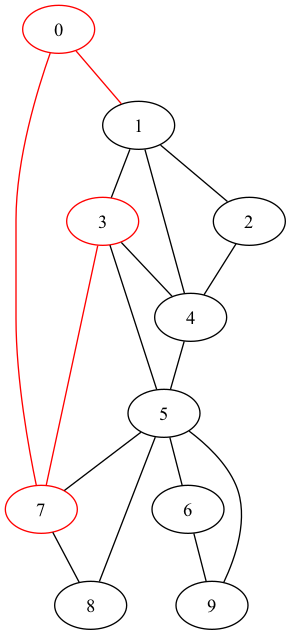
\includegraphics[height=0.29\textheight]{notebook/assets/aufgabe_07_fleury_step_2.png}
        \caption{Step 3}
        \label{fig:fleury_step_3}
    \end{subfigure}
    
    \vspace{1em}
    
    \begin{subfigure}[b]{0.3\textwidth}
        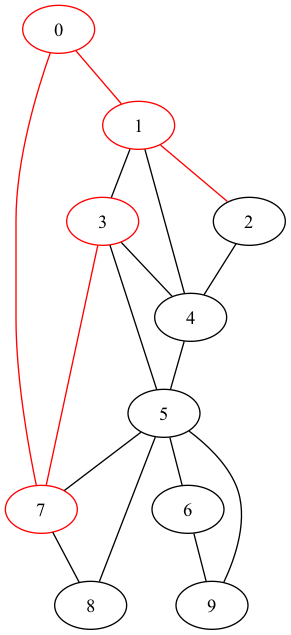
\includegraphics[height=0.29\textheight]{notebook/assets/aufgabe_07_fleury_step_3.png}
        \caption{Step 4}
        \label{fig:fleury_step_4}
    \end{subfigure}
    \hfill
    \begin{subfigure}[b]{0.3\textwidth}
        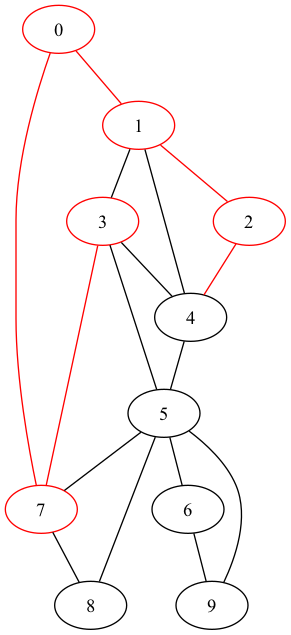
\includegraphics[height=0.29\textheight]{notebook/assets/aufgabe_07_fleury_step_4.png}
        \caption{Step 5}
        \label{fig:fleury_step_5}
    \end{subfigure}
    \hfill
    \begin{subfigure}[b]{0.3\textwidth}
        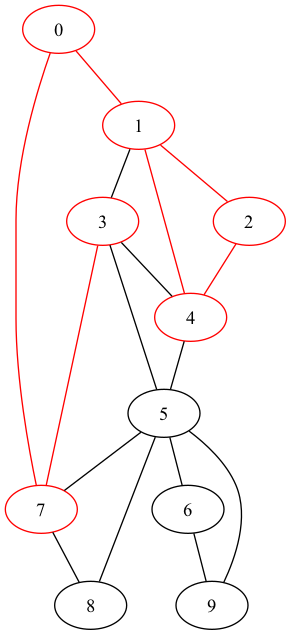
\includegraphics[height=0.29\textheight]{notebook/assets/aufgabe_07_fleury_step_5.png}
        \caption{Step 6}
        \label{fig:fleury_step_6}
    \end{subfigure}
    
    \vspace{1em}
    
    \begin{subfigure}[b]{0.3\textwidth}
        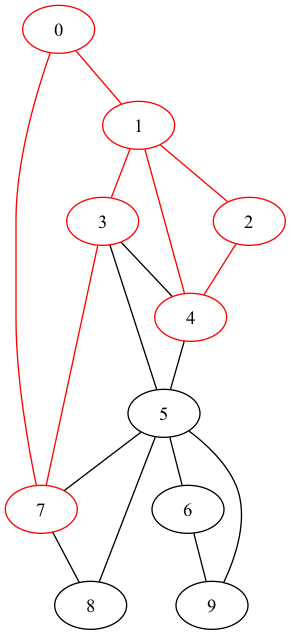
\includegraphics[height=0.29\textheight]{notebook/assets/aufgabe_07_fleury_step_6.png}
        \caption{Step 7}
        \label{fig:fleury_step_7}
    \end{subfigure}
    \hfill
    \begin{subfigure}[b]{0.3\textwidth}
        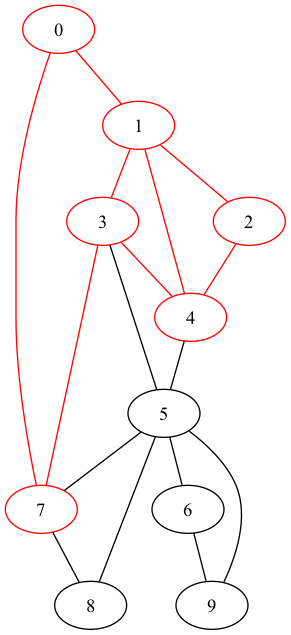
\includegraphics[height=0.29\textheight]{notebook/assets/aufgabe_07_fleury_step_7.png}
        \caption{Step 8}
        \label{fig:fleury_step_8}
    \end{subfigure}
    \hfill
    \begin{subfigure}[b]{0.3\textwidth}
        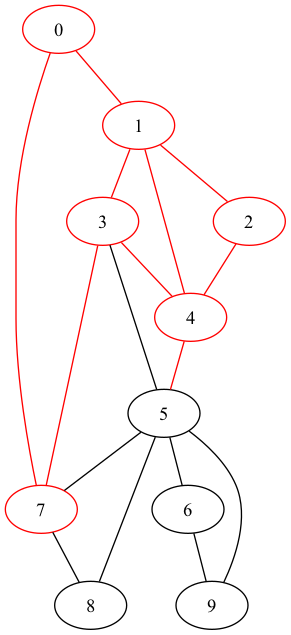
\includegraphics[height=0.29\textheight]{notebook/assets/aufgabe_07_fleury_step_8.png}
        \caption{Step 9}
        \label{fig:fleury_step_9}
    \end{subfigure}
    
    \caption{Fleury Algorithm Steps}
    \label{fig:fleury_algorithm_steps}
\end{figure}

\newpage

\chapter{Euler und Hamilton}
Falls möglich beschreiben Sie \underline{jeweils} einen zusammenhängenden Graphen mit Ordnung $\geq 3$ der

\begin{enumerate}[label=\alph*.]
    \item keinen Eulerkreis und keinen Hamiltonkreis
    \begin{figure}[htbp]
        \centering
        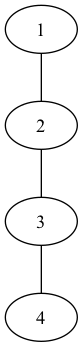
\includegraphics[height=2.5cm]{notebook/assets/aufgabe_08_graph_a.png}
        \caption{Kein Eulerkreis und kein Hamiltonkreis}
        \label{fig:no_euler_no_hamilton}
    \end{figure}
    \item einen Eulerkreis, aber keinen Hamiltonkreis
    \begin{figure}[htbp]
        \centering
        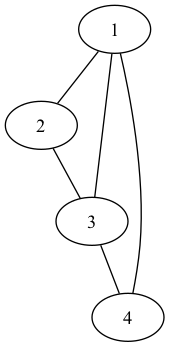
\includegraphics[height=2.5cm]{notebook/assets/aufgabe_08_graph_b.png}
        \caption{Ein Eulerkreis, aber kein Hamiltonkreis}
        \label{fig:neuler_no_hamilton}
    \end{figure}
    \item keinen Eulerkreis, aber einen Hamiltonkreis
    \begin{figure}[htbp]
        \centering
        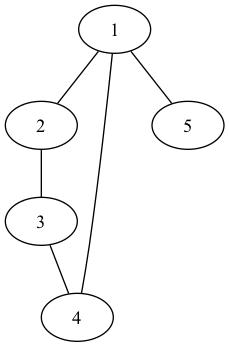
\includegraphics[height=2.5cm]{notebook/assets/aufgabe_08_graph_c.png}
        \caption{Kein Eulerkreis, aber ein Hamiltonkreis}
        \label{fig:no_euler_hamilton}
    \end{figure}
    \item einen Eulerkreis und einen Hamiltonkreis
    \begin{figure}[htbp]
        \centering
        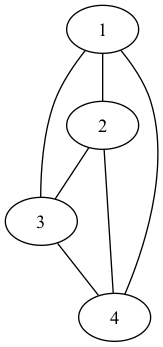
\includegraphics[height=2.5cm]{notebook/assets/aufgabe_08_graph_d.png}
        \caption{Ein Eulerkreis und ein Hamiltonkreis}
        \label{fig:euler_hamilton}
    \end{figure}
\end{enumerate}

aufweist.

\newpage

\chapter{Legal}
Die Ausarbeitung der Aufgabe wurde durch \texttt{OpenAI - GPT-4.5 Turbo}, \texttt{OpenAI - GPT-4.5 Vision}, \texttt{Anthropic -- Claude 3 Opus},  \texttt{Kagi - FastGPT} mit mehreren unterschiedlichen Prompts und Custom Instructions unterstützt.

\end{document}